% -*- Mode:TeX -*-
%% Stefan Negru -- blankdots.com -- An adaption of MIT Thesis format fo
%% Faculty of Computer Science, Alexandru Ioan Cuza University

%% IMPORTANT: The official MIT thesis specifications are available at:
%%            http://libraries.mit.edu/archives/thesis-specs/
%%
%%            Please verify your thesis' formatting and copyright
%%            assignment before submission. 

%% The documentclass options along with the pagestyle can be used to generate
%% a technical report, a draft copy, or a regular thesis.  You may need to
%% re-specify the pagestyle after you \include  cover.tex.  For more
%% information, see the first few lines of mitthesis.cls. 

%\documentclass[12pt,vi,twoside]{mitthesis}
%%
%%  If you want your thesis copyright to you instead of MIT, use the
%%  ``vi'' option, as above.
%%
%\documentclass[12pt,twoside,leftblank]{mitthesis}
%%
%% If you want blank pages before new chapters to be labelled ``This
%% Page Intentionally Left Blank'', use the ``leftblank'' option, as
%% above. 

\documentclass[11pt,twoside]{mitthesis}
\special{papersize=210mm,297mm}
\usepackage{lgrind}

%%%%%%%%%% BEGIN custom settings to the format %%%%%%%%%% 
%\usepackage{minitoc} -- does not work with titlesec
\usepackage{titlesec} % fancy chapter titles and mini ToC
\usepackage{titletoc}
% BEGIN generate nice figures with eps files
\usepackage{graphicx}
\usepackage{epstopdf}
\usepackage{epsfig}
% END generate nice figures with eps files
\usepackage{array} % defines new options for column alignment like "m{width}"
\usepackage{url} % URL package
\usepackage[backref=page]{hyperref} %package for references; PRO TIP: use \autoref
\usepackage[hypcap]{caption}
\usepackage{amsthm, amsfonts, amsmath, amssymb} % math, definitions stuff
\usepackage[nottoc]{tocbibind} % disable inclusion of ToC in ToC; notbib disables bibliography in ToC
\usepackage{listings} % for source code listing
\usepackage{enumitem}
\usepackage{emptypage} %clear empty pages from page numbering
\usepackage{wrapfig} % for inline image placement
%\usepackage{paralist} % for inline enumeration

\RequirePackage[absolute]{textpos}

% Uncomment to set hyperef colors in the pdf for digital document
\hypersetup{colorlinks=true, urlcolor=blue, linkcolor=blue, citecolor=red, pdfborder={0 0 0}}

% Uncomment to set hyperef colors for print format
%\hypersetup{colorlinks=true, urlcolor=black, linkcolor=black, citecolor=black, pdfborder={0 0 0}}

% set back references in the bibliography to see on which page that specific reference was cited
\renewcommand*{\backref}[1]{}
\renewcommand*{\backrefalt}[4]{%
    \ifcase #1 (Not cited.)%
    \or        (Cited on page~#2.)%
    \else      (Cited on pages~#2.)%
    \fi}

%---- For theorems, definitions and examples
\theoremstyle{definition}
\newtheorem{theorem}{Theorem}[section]
\newtheorem{example}{Example}[section]
\newtheorem{definition}{Definition}[section]
\newtheorem{exercise}[theorem]{Exercise}

%----correct case for autoref from hyperref
\renewcommand*{\chapterautorefname}{Chapter}
\renewcommand*{\sectionautorefname}{Section}%
\providecommand*{\lstnumberautorefname}{Listing}
\newcommand{\exampleautorefname}{Example}
\newcommand{\definitionautorefname}{Definition}

% Formatting for Chapter Titles and beginning of Chapters
%----\RequirePackage{titlesec}

\titleformat{\chapter}[display]
  {\normalfont\Large\raggedleft}
  {\MakeUppercase{\chaptertitlename}%
    \rlap{ \resizebox{!}{1.2cm}{\thechapter} \rule{15cm}{1.2cm}}}
  {7pt}{\Huge}
\titlespacing*{\chapter}{0pt}{30pt}{20pt}

\AtBeginDocument{\renewcommand\contentsname{Table of Contents}}

%---- pagestyle header for pagenumber and chapter title
\newpagestyle{special}{
  \headrule
  \sethead[\small{\usepage}][\small{\chaptertitle}]
	     []{}{\small{\chaptertitle}}{\small{\usepage}}
}

%---- fix for conflict with minitoc; creating partial TOC for each chapter

\newcommand{\PartialToc}{\vspace*{1pc}\vbox{\bf\Large Contents\vspace*{1pc}}%
\startcontents[chapters]\hrule\vspace*{1pc}
\printcontents[chapters]{}{1}{\setcounter{tocdepth}{1}}\vspace*{1pc}\hrule\vspace*{1pc}}

\lstset{basicstyle=\small\ttfamily,breaklines=true} %listing monospace font formating

%%%%%%%%%% END custom settings to the format %%%%%%%%%% 

\def\all{all}

\begin{document}

\pagestyle{plain}

%% Stefan Negru -- blankdots.com -- An adaption of MIT Thesis format for
%% Faculty of Computer Science, Alexandru Ioan Cuza University
% -*-latex-*-

\title{Thesis Title}

\author{FirstName LastName}
% If you wish to list your previous degrees on the cover page, use the
% previous degrees command:
%       \prevdegrees{B.Sc., Faculty of Computer Science (2008)}
% You can use the \\ command to list multiple previous degrees
%       \prevdegrees{M.Sc., Faculty of Computer Science (2010)}
\department{Faculty of Computer Science}

% If the thesis is for two degrees simultaneously, list them both
% separated by \and like this:
% \degree{Doctor of Philosophy \and Master of Science}
\degree{Bachelor/Master/Philosophiae Doctor}

% As of the 2007-08 academic year, valid degree months are September,
% February, or June.  The default is June.
\degreemonth{Month}
\degreeyear{Year}
\thesisdate{Month DD, Year}

%% By default, the thesis will be copyrighted to MIT.  If you need to copyright
%% the thesis to yourself, just specify the `vi' documentclass option.  If for
%% some reason you want to exactly specify the copyright notice text, you can
%% use the \copyrightnoticetext command.
%\copyrightnoticetext{\copyright blankdots, 2013. Do not open till Xmas.}

% If there is more than one supervisor, use the \supervisor command
% once for each.
\supervisor{Professor FirstName Lastname}

% This is the department committee chairman, not the thesis committee
% chairman.  You should replace this with your Department's Committee
% Chairman.
%\chairman{Arthur C. Smith}{Chairman, Department Committee on Graduate Theses}

% Make the titlepage based on the above information.  If you need
% something special and can't use the standard form, you can specify
% the exact text of the titlepage yourself.  Put it in a titlepage
% environment and leave blank lines where you want vertical space.
% The spaces will be adjusted to fill the entire page.  The dotted
% lines for the signatures are made with the \signature command.
\maketitle

% The abstractpage environment sets up everything on the page except
% the text itself.  The title and other header material are put at the
% top of the page, and the supervisors are listed at the bottom.  A
% new page is begun both before and after.  Of course, an abstract may
% be more than one page itself.  If you need more control over the
% format of the page, you can use the abstract environment, which puts
% the word "Abstract" at the beginning and single spaces its text.

%% You can either \input (*not* \include) your abstract file, or you can put
%% the text of the abstract directly between the \begin{abstractpage} and
%% \end{abstractpage} commands.

% First copy: start a new page, and save the page number.
\cleardoublepage
% Uncomment the next line if you do NOT want a page number on your
% abstract and acknowledgments pages.
\pagestyle{empty}
%\setcounter{savepage}{\thepage}
\begin{abstractpage}
%% Stefan Negru -- blankdots.com -- An adaption of MIT Thesis format fo
%% Faculty of Computer Science, Alexandru Ioan Cuza University

%% The text of your abstract and nothing else (other than comments) goes here.
%% It will be single-spaced and the rest of the text that is supposed to go on
%% the abstract page will be generated by the abstractpage environment.  This
%% file should be \input (not \include 'd) from cover.tex.

Abstract for the thesis goes here. The abstract was designed for students from Faculty of Computer Science, Alexandru Ioan Cuza University but feel free to adapt and modify. 

This LaTeX form is adapted form the MIT Thesis format available at \url{http://web.mit.edu/thesis/tex/}.

Also consult the guide available at \url{http://profs.info.uaic.ro/~mdiac/other/licenta2010/ghid_licenta2010.pdf}

\vspace{0.5cm}

\textbf{Keywords:} Thesis Format, LaTeX, Example

\end{abstractpage}

% Additional copy: start a new page, and reset the page number.  This way,
% the second copy of the abstract is not counted as separate pages.
% Uncomment the next 6 lines if you need two copies of the abstract
% page.
% \setcounter{page}{\thesavepage}
% \begin{abstractpage}
% %% Stefan Negru -- blankdots.com -- An adaption of MIT Thesis format fo
%% Faculty of Computer Science, Alexandru Ioan Cuza University

%% The text of your abstract and nothing else (other than comments) goes here.
%% It will be single-spaced and the rest of the text that is supposed to go on
%% the abstract page will be generated by the abstractpage environment.  This
%% file should be \input (not \include 'd) from cover.tex.

Abstract for the thesis goes here. The abstract was designed for students from Faculty of Computer Science, Alexandru Ioan Cuza University but feel free to adapt and modify. 

This LaTeX form is adapted form the MIT Thesis format available at \url{http://web.mit.edu/thesis/tex/}.

Also consult the guide available at \url{http://profs.info.uaic.ro/~mdiac/other/licenta2010/ghid_licenta2010.pdf}

\vspace{0.5cm}

\textbf{Keywords:} Thesis Format, LaTeX, Example

% \end{abstractpage}

\cleardoublepage

% Delete the section below for it not to be included in the paper

\section*{Acknowledgments}

Lorem ipsum dolor sit amet, consectetur adipiscing elit. In nunc mi, iaculis vel arcu quis, eleifend semper dolor. Aliquam pretium consectetur dui eu accumsan. Nulla facilisi. Nunc sodales at velit vitae ultricies. Pellentesque habitant morbi tristique senectus et netus et malesuada fames ac turpis egestas. Morbi semper et enim ut pretium. Donec sit amet metus sed nulla ullamcorper feugiat id id dui. In imperdiet neque dolor, ac imperdiet elit sagittis non. Mauris non leo at mi tempus adipiscing.
%%%%%%%%%%%%%%%%%%%%%%%%%%%%%%%%%%%%%%%%%%%%%%%%%%%%%%%%%%%%%%%%%%%%%%
% -*-latex-*-
\cleardoublepage


\pagenumbering{roman} % roman page numbering system
  % -*- Mode:TeX -*-
%% This file simply contains the commands that actually generate the table of
%% contents and lists of figures and tables.  You can omit any or all of
%% these files by simply taking out the appropriate command.  For more
%% information on these files, see appendix C.3.3 of the LaTeX manual.

\tableofcontents
%\newpage
\listoffigures
%\newpage
\listoftables

 % table of contents, list of figures, list of tables
%% Stefan Negru -- blankdots.com -- An adaption of MIT Thesis format fo
%% Faculty of Computer Science, Alexandru Ioan Cuza University

%%% List of published papers and personal contributions %%%

% --- Quick fix to unlist chapter
\chapter*{List of Contributions} % use '*' to unlist chapter for TOC
\addcontentsline{toc}{chapter}{List of Contributions}
\label{chap:Articles}

\begin{enumerate}
	\item \textbf{Contribution 1}. Lorem ipsum dolor sit amet, consectetur adipiscing elit. In faucibus diam gravida malesuada feugiat. Sed pharetra bibendum nunc, sed interdum erat hendrerit a.
\end{enumerate}

\noindent End of the list of personal contributions followed by a personal statement regarding the importance of the contributions.

\cleardoublepage % list of publications and personal contributions

%% Stefan Negru -- blankdots.com -- An adaption of MIT Thesis format for
%% Faculty of Computer Science, Alexandru Ioan Cuza University

\newpage
\thispagestyle{empty}

\section*{Declara\c tie Privind Originalitatea \c si Respectarea Drepturilor de Autor}

\noindent Prin prezenta declar c\u a Lucrarea de Licen\c t\u a / Master cu titlul \textbf{Titlul Complet} este scris\u a de mine \c si nu a mai fost prezentat\u a niciodat\u a la o alta facultate sau institu\c tie de \^inv\u a\c t\u am\^ant superior din \c tar\u a sau str\u ain\u atate. De asemenea, declar c\u a toate sursele utilizate, inclusiv cele preluate de pe Internet sunt indicate \^in lucrare, cu respectarea regulilor de evitare a plagiatului:

\begin{itemize}
	\item toate fragmentele de text reproduse exact, chiar \c si \^in traducere proprie din alt\u a limb\u a, sunt scrise \^intre ghilimele \c si de\c tin referin\c ta precis\u a a sursei;
	\item reformularea \^in cuvinte proprii a textelor scrise de c\u atre al\c ti autori de\c tine referin\c ta precis\u a;
	\item codul surs\u a, imagini etc. preluate din proiecte \textit{open-source} sau alte resurse sunt utilizate cu respectarea drepturilor de autor \c si de\c tin referin\c te precise;
	\item rezumarea ideilor altor autori precizeaz\u a referin\c ta precis\u a la textul original.
\end{itemize}

\vspace{10 mm}

\noindent\begin{tabular}{p{8cm}r}
Ia\c si, Data & Absolvent Prenume Nume\\[8ex]
	 & \makebox[2.5in]{\hrulefill}\\
 & (semn\u atura \^in original)\\% adds space between the two sets of signatures

\end{tabular}

%% ------------------------------ %%

\newpage
\thispagestyle{empty}

\section*{Declara\c tie de Consin\c t\u am\^ant}

\noindent Prin prezenta declar c\u a sunt de acord ca Lucrarea de Licen\c t\u a / Master cu titlul \textbf{Titlul Complet}, codul surs\u a al programelor \c si celelate con\c tinuturi (grafice, multimedia, date de test etc.) care \^inso\c tesc aceast\u a lucrare s\u a fie utilizate \^in cadrul Facult\u a\c tii de Informatic\u a.

\noindent De asemenea, sunt de acord ca Facultatea de Informatic\u a de la Universitatea Alexandru Ioan Cuza, Ia\c si s\u a utilizeze, modifice, reproduc\u a \c si s\u a distribuie \^in scopuri necomerciale aplica\c tiile, codul surs\u a, executabilele \c si documenta\c tia, realizate de mine \^in cadrul prezentei lucr\u ari.

\vspace{10 mm}

\noindent\begin{tabular}{p{8cm}r}
Ia\c si, Data & Absolvent Prenume Nume\\[8ex]
	 & \makebox[2.5in]{\hrulefill}\\
 & (semn\u atura \^in original)\\% adds space between the two sets of signatures

\end{tabular}

%% ------------------------------ %%

\newpage
\thispagestyle{empty}

\section*{Acord Privind Proprietatea Dreptului de Autor}

\noindent Facultatea de Informatic\u a este de acord ca drepturile de autor asupra aplica\c tiilor, codului surs\u a, executabilelor \c si documenta\c tiei, s\u a apar\c tin\u a autorului prezentei lucr\u ari \textit{Prenume Nume}.

\noindent \^Incheierea acestui acord este necesar\u a din urm\u atoarele motive:

\textit{Se explic\u a de ce este necesar un acord, se descriu originile resurselor utilizate \^in realizarea produsului-program (personal, tehnologii, fonduri) \c si aportul adus de fiecare resurs\u a.}

\vspace{10 mm}

\noindent\begin{tabular}{p{8cm}r}
Ia\c si, Data & \\[8ex]
Decan, Prenume Nume & Absolvent Prenume Nume \\
\makebox[2.5in]{\hrulefill}	& \makebox[2.5in]{\hrulefill}\\
(semn\u atura \^in original) & (semn\u atura \^in original)\\% adds space between the two sets of signatures

\end{tabular}

\cleardoublepage
 % declarations for Romanian students -- remove if not needed

\pagenumbering{arabic} % arabic page numbering system
\pagestyle{special}

%% Stefan Negru -- blankdots.com -- An adaption of MIT Thesis format fo
%% Faculty of Computer Science, Alexandru Ioan Cuza University

%% A chapter

\chapter{Introduction}
\label{chap:Introduction}
\PartialToc % Include partial Table of contents for each Chapter

Lorem ipsum dolor sit amet \cite{Name2014}, consectetur adipiscing elit. In nunc mi, iaculis vel arcu quis, eleifend semper dolor. Aliquam pretium consectetur dui eu accumsan. Nulla facilisi. Nunc sodales at velit vitae ultricies. Pellentesque habitant morbi tristique senectus et netus et malesuada fames ac turpis egestas. Morbi semper et enim ut pretium. Donec sit amet metus sed nulla ullamcorper feugiat id id dui. In imperdiet neque dolor, ac imperdiet elit sagittis non. Mauris non leo at mi tempus adipiscing. 

%----------------------------------------------------------

\section{Structure}

 Lorem ipsum dolor sit amet, consectetur adipiscing elit. In nunc mi, iaculis vel arcu quis, eleifend semper dolor. Aliquam pretium consectetur dui eu accumsan. Nulla facilisi. Nunc sodales at velit vitae ultricies. Pellentesque habitant morbi tristique senectus et netus et malesuada fames ac turpis egestas. Morbi semper et enim ut pretium. Donec sit amet metus sed nulla ullamcorper feugiat id id dui. In imperdiet neque dolor, ac imperdiet elit sagittis non. Mauris non leo at mi tempus adipiscing.

Integer malesuada ullamcorper nulla (\autoref{chap:Introduction}), in commodo nisi porta at. Praesent diam sapien, volutpat id magna dignissim, ultricies dictum dolor. Vestibulum ultrices metus porta sem viverra, quis volutpat leo hendrerit. Phasellus lacus nibh, lacinia eu nulla sed, imperdiet dapibus felis. Aliquam mattis commodo eros pulvinar faucibus. Sed gravida lorem sed condimentum gravida. Suspendisse quis semper lorem. Cras purus nibh, interdum eget est in, convallis porttitor arcu. Aliquam suscipit turpis in tempus cursus. In iaculis tortor volutpat urna ullamcorper elementum. Mauris elementum metus id arcu pretium sollicitudin. Ut convallis ut nisi nec commodo. Nam ligula risus, lobortis ac auctor sed, lobortis vel felis. Integer dapibus molestie purus, a suscipit sem posuere quis. Ut lobortis lacus et lectus vehicula, sed iaculis massa consectetur. 

%----------------------------------------------------------

\section{Contributions}
\label{sec:ObjectiveContributions}


\textbf{Aliquam} dignissim vel diam in facilisis. Morbi pulvinar massa non porttitor adipiscing. Aenean tincidunt in orci et eleifend. Sed vel gravida velit, at pretium mauris. Aenean eros magna, rhoncus eget ipsum et, accumsan dapibus elit. Donec \textit{quis ultricies tortor}, et tempus neque. Cras suscipit, lorem eget semper condimentum, tellus diam fringilla sapien, sed tempus justo arcu vel tortor. 

\begin{itemize}[noitemsep]
	\item Lorem ipsum dolor sit amet, consectetur adipiscing elit.;
	\item Vivamus molestie tellus eget arcu eleifend laoreet;
	\item Phasellus venenatis risus eleifend augue sagittis semper;
	\item Integer bibendum risus non dolor sagittis, sed vestibulum nibh dictum. (\autoref{chap:AppendixA});
	\item Maecenas sollicitudin nisi a nisi rhoncus, ac fringilla leo malesuada. (\autoref{sec:Other}).
\end{itemize}


\begin{itemize}[noitemsep]
    \item Cras dapibus mi vitae tristique faucibus.
    \item Ut tristique leo nec erat eleifend viverra.
    \item Made by -- \url{http://blankdots.com}.
    .
\end{itemize}

\begin{figure}[h]
		\centering
		{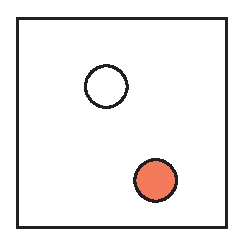
\psfig{file = figures/sample.eps, width =6cm}}
		\caption{Sample Figure.}
		\label{fig:sample}
\end{figure}
Etiam orci leo, euismod ac mattis a (\autoref{fig:sample}), dictum et tellus. In aliquet, neque sed hendrerit lobortis, metus metus lobortis turpis, in molestie turpis tortor commodo tortor. Morbi dapibus nec odio facilisis dignissim. Donec pharetra elit magna, vitae aliquet mauris ultricies tincidunt. Integer vitae lectus sodales, interdum arcu iaculis, mollis lacus. Curabitur luctus quis velit vitae fringilla. Vestibulum pharetra dui ac neque aliquet bibendum. Quisque sit amet luctus erat. Praesent a hendrerit dolor. Cras semper egestas enim. 

%----------------------------------------------------------

\section{Other}
\label{sec:Other}

Nam eu orci ac eros commodo mattis pellentesque sollicitudin lorem. Quisque congue, risus vel fringilla varius, mauris lacus fermentum erat, vel imperdiet libero magna non orci. Etiam cursus dictum lorem vitae cursus. Nunc in justo sed turpis ultricies auctor. Aliquam iaculis fermentum volutpat. Aenean purus purus, condimentum id sapien vel, accumsan ornare tellus. Morbi vulputate placerat lacus, ut rhoncus eros condimentum a. Morbi condimentum gravida sapien at scelerisque. Vivamus feugiat nisi et neque iaculis, quis fermentum orci viverra. Nulla facilisi. 

\subsection{Another}

Integer mollis a sapien eu malesuada. Nam et viverra est, at laoreet magna. In hac habitasse platea dictumst. Sed vitae mauris sem. Sed feugiat quam eget rhoncus vehicula. Ut tellus nisl, cursus non odio in, consequat tempus ipsum. Class aptent taciti sociosqu ad litora torquent per conubia nostra, per inceptos himenaeos. Ut euismod nec turpis ut lobortis. In hac habitasse platea dictumst. Nullam dolor est, blandit eget consequat vitae, porttitor eu elit. Vestibulum ante ipsum primis in faucibus orci luctus et ultrices posuere cubilia Curae; Fusce dictum tellus leo, a dignissim elit sodales facilisis. 

\subsubsection{Another and More}

Lorem ipsum dolor sit amet, consectetur adipiscing elit. In faucibus diam gravida malesuada feugiat. Sed pharetra bibendum nunc, sed interdum erat hendrerit a. Pellentesque gravida ipsum at augue sagittis convallis. Morbi viverra, nunc eu eleifend dignissim, elit nunc gravida tellus, sed eleifend purus tellus a lorem. Aliquam fringilla convallis mollis. Duis vel metus non diam eleifend tempus. Vivamus metus velit, euismod sit amet neque et, tristique eleifend orci. Nulla varius tristique mollis. Duis vitae mauris non ipsum egestas gravida. Ut suscipit nulla lobortis, congue neque sit amet, consequat quam. Quisque sit amet mauris et metus molestie vestibulum at non mauris.  %chapter 1
%% Stefan Negru -- blankdots.com -- An adaption of MIT Thesis format for
%% Faculty of Computer Science, Alexandru Ioan Cuza University

\chapter{Another Chapter Example}
\label{chap:Chapter}
\PartialToc % Include partial Table of contents for each Chapter

%----------------------------------------------------------

\section{General Directions}

Etiam vulputate elit\cite{Weiser1991} a sem lacinia commodo. Nulla vitae tellus bibendum, aliquam augue sed, tincidunt nulla. Vivamus mollis ut magna ac tempor. Vivamus interdum consequat dapibus. Donec sagittis mauris ut vehicula gravida. Nulla fermentum facilisis mollis. Proin hendrerit venenatis orci ut porta. Etiam suscipit libero sapien, non suscipit dolor tincidunt eu. Pellentesque nec sagittis ipsum, sed pellentesque sapien. Nam tempor risus nec vestibulum convallis. Proin eget ornare purus, eget sagittis massa. Donec euismod facilisis metus, placerat auctor quam rhoncus at.


\begin{table}
\small
\renewcommand{\arraystretch}{1.3}
\centering
\caption{Example of namespaces, their URIrefs and prefixes.}
\begin{tabular}{|l|l|c|} \hline
    Namespace & URIref & Prefix \\ \hline
    \hline
	RDF & \url{http://www.w3.org/1999/02/22-rdf-syntax-ns#} & rdf \\ \hline
	RDF Schema & \url{http://www.w3.org/2000/01/rdf-schema#} & rdfs \\ \hline
	XML Schema & \url{http://www.w3.org/2001/XMLSchema} & xsd \\ \hline
	OWL & \url{http://www.w3.org/2002/07/owl#} & owl \\ \hline
	PROV-O & \url{http://www.w3.org/TR/prov-o/} & prov-o \\ \hline
	Dublin Core & \url{http://purl.org/dc/elements/1.1/} & dc \\ \hline
	FOAF & \url{http://xmlns.com/foaf/spec/} & foaf \\ \hline
	MUTO & \url{http://purl.org/muto/core} & muto \\ \hline
	PersonasOnto & \url{http://blankdots.com/open/personasonto.owl} & pont \\
	\hline
\end{tabular}
\label{tab:Namespaces}
\end{table}

\begin{wrapfigure}{l}{0.5\textwidth}
  \begin{center}
		{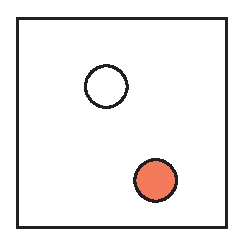
\psfig{file = figures/sample.eps, width = 3cm}}
		\caption{Sample In line.}
	\end{center}
\label{fig:InlineSample}
\end{wrapfigure}

 Lorem ipsum dolor sit amet, consectetur adipiscing elit. In faucibus diam gravida malesuada feugiat. Sed pharetra bibendum nunc, sed interdum erat hendrerit a. Pellentesque gravida ipsum at augue sagittis convallis. Morbi viverra, nunc eu eleifend dignissim, elit nunc gravida tellus, sed eleifend purus tellus a lorem. Aliquam fringilla convallis mollis. Duis vel metus non diam eleifend tempus. Vivamus metus velit, euismod sit amet neque et, tristique eleifend orci. Nulla varius tristique mollis. Duis vitae mauris non ipsum egestas gravida. Ut suscipit nulla lobortis, congue neque sit amet, consequat quam. Quisque sit amet mauris et metus molestie vestibulum at non mauris.

Etiam orci leo, euismod ac mattis a, dictum et tellus. In aliquet, neque sed hendrerit lobortis, metus metus lobortis turpis, in molestie turpis tortor commodo tortor. Morbi dapibus nec odio facilisis dignissim. Donec pharetra elit magna, vitae aliquet mauris ultricies tincidunt. Integer vitae lectus sodales, interdum arcu iaculis, mollis lacus. Curabitur luctus quis velit vitae fringilla. Vestibulum pharetra dui ac neque aliquet bibendum. Quisque sit amet luctus erat. Praesent a hendrerit dolor. Cras semper egestas enim.

%----------------------------------------------------------

\section{Conclusions}

Lorem ipsum dolor sit amet\footnote{\url{http://www.w3.org/1998/02/Potential.html}}, consectetur adipiscing elit. In faucibus diam gravida malesuada feugiat. Sed pharetra bibendum nunc, sed interdum erat hendrerit a. Pellentesque gravida ipsum at augue sagittis convallis. Morbi viverra, nunc eu eleifend dignissim, elit nunc gravida tellus, sed eleifend purus tellus a lorem. Aliquam fringilla convallis mollis. Duis vel metus non diam eleifend tempus. Vivamus metus velit, euismod sit amet neque et, tristique eleifend orci. Nulla varius tristique mollis. Duis vitae mauris non ipsum egestas gravida. Ut suscipit nulla lobortis, congue neque sit amet, consequat quam. Quisque sit amet mauris et metus molestie vestibulum at non mauris.

Etiam orci leo, euismod ac mattis a, dictum et tellus. In aliquet, neque sed hendrerit lobortis, metus metus lobortis turpis, in molestie turpis tortor commodo tortor. Morbi dapibus nec odio facilisis dignissim. Donec pharetra elit magna, vitae aliquet mauris ultricies tincidunt. Integer vitae lectus sodales, interdum arcu iaculis, mollis lacus. Curabitur luctus quis velit vitae fringilla. Vestibulum pharetra dui ac neque aliquet bibendum. Quisque sit amet luctus erat. Praesent a hendrerit dolor. Cras semper egestas enim.
 %chapter 2

\pagestyle{plain}
\appendix
%% Stefan Negru -- blankdots.com -- An adaption of MIT Thesis format for
%% Faculty of Computer Science, Alexandru Ioan Cuza University

\chapter{Appendix Example}
\label{chap:AppendixA}

\begin{table}[h]
\centering
\renewcommand{\arraystretch}{1}
\caption{OWL DL descriptions, data ranges, properties, individuals, and data values; content adapted from \cite{Baader2003}.}
\begin{tabular}{|p{10cm}|p{5cm}|}
	\multicolumn{1}{l}{\textbf{Abstract Syntax}}
	& \multicolumn{1}{l}{\textbf{DL Syntax}}\\
			\hline
			Descriptions ($C$) & {}\\
			\hline
			A & A\\
			owl:Thing & $\top$\\
			owl:Nothing & $\bot$\\
		 \hline
			intersectionOf $(C_{1}\ldots C_{n})$ & $C_{1}\sqcap \cdots \sqcap C_{n}$ \\
			unionOf $(C_{1}\ldots C_{n})$ & $C_{1}\sqcup \cdots \sqcup C_{n}$ \\
			complementOf $(C)$ & $\neg C$\\
			oneOf $(o_{1} \ldots o_{n})$ & $\{o_{1}\} \sqcup \cdots \sqcup \{o_{n}\}$\\
			\hline
			restriction ($R$ someValuesFrom $(C)$) & $\exists R.C$ \\
			restriction ($R$ allValuesFrom $(C)$) & $\forall R.C$ \\
			restriction ($R$ hasValue $(o)$) & $R:o$ \\
			restriction ($R$ minCardinality $(n)$) & $\ge n$ $R$ \\
			restriction ($R$ maxCardinality $(n)$) & $\le n$ $R$ \\
			\hline
			restriction ($U$ someValuesFrom $(C)$) & $\exists U.C$ \\
			restriction ($U$ allValuesFrom $(C)$) & $\forall U.C$ \\
			restriction ($U$ hasValue $(v)$) & $U:v$ \\
			restriction ($U$ minCardinality $(n)$) & $\ge n$ $U$ \\
			restriction ($U$ maxCardinality $(n)$) & $\le n$ $U$ \\
			\hline
			\hline
			Data Ranges ($D$) & {}\\
			\hline
			D & D\\
			oneOf $(v_{1} \cdots v_{n})$ & $\{o_{1}\} \sqcup \cdots \sqcup \{v_{n}\}$\\
			\hline
			Object Properties($R$) & {}\\
			\hline
			R & R\\
			inv$(R)$ & $R^{-}$\\
			\hline
			\hline
			Datatype Properties($U$) & {}\\
			\hline
			U & U\\
			\hline
			\hline
			Individuals($o$) & {}\\
			\hline
			o & o\\
			\hline
			\hline
			Data Values($v$) & {}\\
			\hline
			v & v\\
			\hline
		\end{tabular}
\label{tab:OWLvsDL}
\end{table}
 % appendix
%% Stefan Negru -- blankdots.com -- An adaption of MIT Thesis format for
%% Faculty of Computer Science, Alexandru Ioan Cuza University

%% This defines the bibliography file (main.bib) and the bibliography style.
%% If you want to create a bibliography file by hand, change the contents of
%% this file to a `thebibliography' environment.  For more information
%% see section 4.3 of the LaTeX manual.
\begin{singlespace}
\bibliography{main}
\bibliographystyle{plain}
\end{singlespace}

\end{document}

